\chapter{Quadrotor based object follow control algorithm}

	\section{Quadrotor Model}
	\label{sec:Quadrotor Model}
	
	This section shows the 6-DOF model of a quadrotor based on rigid body dynamics. The derivation of kinematic equations are followed by the derivation
	of dynamic equations.~\cite{drone}
	
	\subsection{Kinematics}
	\label{sec:Kinematics}
	For describing the dynamics of a rigid body we use 2 coordinate frames
	i.e., the inertial and body fixed coordinates. All the physical quantities are
	transferred between the two coordinate system using the well known Euler
	angles ($\phi -$ roll, $\theta -$ −pitch, $\psi -$ −yaw). The following expression relates the velocity of quadrotor the two frames:
	
	\begin{equation}
	\frac{d}{dt}\begin{pmatrix}
	x\\y\\z
	\end{pmatrix} = R^{v}_b\begin{pmatrix}
	u\\v\\w
	\end{pmatrix}
	\end{equation}
	where,
	\begin{equation}
	R^{v}_b = \begin{pmatrix}
	cos\theta cos\psi & sin\phi sin\theta cos\psi - cos\phi sin\psi & cos\phi sin\theta cos\psi + sin\phi sin\psi \\
	cos\theta sin\psi & sin\phi sin\theta sin\psi + cos\phi cos\psi & cos\phi sin\theta sin\psi - sin\phi cos\psi \\
	- sin\theta & sin\phi cos\theta & cos\phi cos\theta
	\end{pmatrix}
	\end{equation}
	
	Here u,v,w are the velocity coordinates in the body frame and x,y,z are the
	velocity coordinates in the inertial frame. Similarly, the following expression
	relates the body rates and Euler angle rates
	\begin{equation}
	\begin{pmatrix}
	\dot{\phi} \\ \dot{\theta} \\ \dot{\psi}
	\end{pmatrix} = \begin{pmatrix}
	1 & sin\phi sin\theta sec\theta & cos\phi sin\theta sec\theta \\
	0 & cos\phi & -sin\phi \\
	0 & sin\phi sec\theta & cos\phi sec\theta
	\end{pmatrix} \begin{pmatrix}
	p \\ q \\ r
	\end{pmatrix}
	\end{equation}
	
	
	\subsection{Dynamics}
	\label{sec: Dynamics}
	
	The dynamical equations for a quadrotor is obtained by applying Newtons second law on a rigid body. The forces acting on a quadrotor can be assumed to be the sum of gravitational force, aerodynamic forces, and propulsion forces. In this work, it is assumed that propulsive force (thrust from the motors) and the gravitational forces are the dominant forces. The aerodynamic force is neglected assuming them to be very small. Transforming the translational dynamics to the inertial frame as follows:
	
	\begin{equation}
	\begin{pmatrix}
	\ddot{x} \\ \ddot{y} \\ \ddot{z}
	\end{pmatrix}
		= R^{i}_b \begin{pmatrix}
		0 \\ 0 \\ \frac{-T}{m}
		\end{pmatrix}
		+ \begin{pmatrix}
		0 \\ 0 \\ g
		\end{pmatrix}
	\end{equation}
	Assuming the quadrotor to be symmetric about x and y axis, the rotational dynamics is given as follows:
	
	\begin{equation}
	\begin{pmatrix}
	\dot{p} \\ \dot{q} \\ \dot{r}
	\end{pmatrix}
	= \begin{pmatrix}
	\frac{I_{yy} - I_{zz}}{I_{xx}} qr \\ \frac{I_{zz} - I_{xx}}{I_{yy}} pr \\ \frac{I_{xx} - I_{yy}}{I_{zz}} pq
	\end{pmatrix}
	+ \begin{pmatrix}
	\frac{l}{I_{xx}} \\ \frac{m}{I_{yy}} \\ \frac{n}{I_{zz}}
	\end{pmatrix}
	\end{equation}
	
	Note that the cross product terms of the inertia matrix are assumed to be
	zero. Here, l, m, and n are the components of the externally applied moments
	known as rolling, pitching, and yawing moments, respectively. All these
	equations together represent the complete six-DOF of a quadrotor.
	
	
	\section{Controller Design}
	\label{sec:Controller Design}
	
	\subsection{PID control}
	\label{sec:PID control}
	
	\makeatletter
	\setlength{\@fptop}{0pt}
	\makeatother
	\begin{figure}[htb]
		\centering
		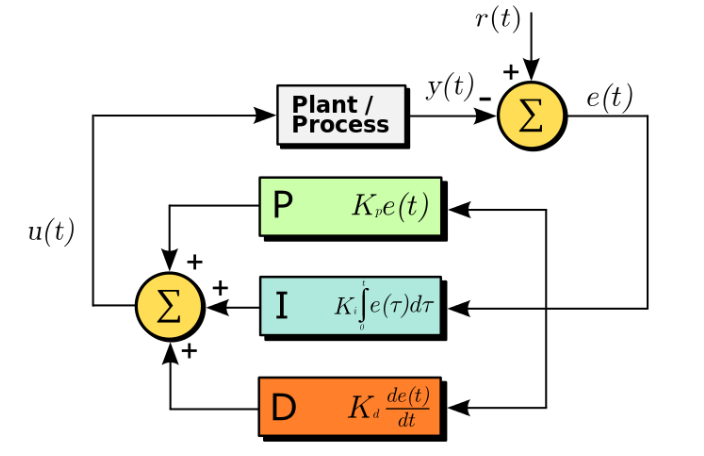
\includegraphics[width=12cm]{pidcontrol.png}
		\caption{PID controller\label{ROS working}}
	\end{figure}
	
	A PID \emph{(Proportional-Intergral-Derivative)} controller is just another type of feedback controller, based on classical control theory. It its most widely used
	controller in industrial applications. It is based on continuously calculating
	the value of an ”error value” between a measured quantity and desired quantity. It then tries to minimize this error over time.
	The basic control law in PID Controller is :
	
	\begin{equation}
	u(t) = K_{p}e(t) + K_{d}\frac{de(t)}{dt} + K_{i}\int_{0}^{t} e(\tau) d\tau
	\end{equation}
	
	where $K_p$ , $K_i$ ,and $K_d$ , all non-negative, denote the coefficients for the proportional, integral, and derivative terms, and $e(t) = r(t)-$$y(t)$, y(t) is measured process variable and r(t) is desired set point.
	
	
	
	\subsection{Implementation in Quadrotors}
	\label{sec:Implementation in Quadrotors}
	
	\subsubsection{Outer Loop}
	
	As we have already seen, the PID controller calculates the value of an error and then try to minimise it. For quadrotor, PIDs are widely used. Solving the kinematic equations [6.1] and [6.2], we get the following,	
	\begin{equation}
	\begin{aligned}
	\ddot{x} = (cos\phi sin\theta cos\psi + sin\phi sin\psi)(-T/m) \\
	\ddot{y} = (cos\phi sin\theta sin\psi + sin\phi cos\psi)(-T/m) \\
	\ddot{z} = (cos\phi cos\theta)(-T/m) + g	\\
	\end{aligned}
	\end{equation}
	
	Assuming small angle approximation, we can actually decouple the system
	to a fair extent. Then we have,
	
	\begin{equation}
	\begin{aligned}
	\ddot{x} = \frac{-T}{m}\theta \\
	\ddot{y} = \frac{T}{m}\phi \\
	\ddot{z} = \frac{-T}{m} + g \\
	\end{aligned}
	\end{equation}
	
	According to PID control law, we write,
	
	\begin{equation}
	\begin{aligned}
	\theta = K_{p_\theta}(x_d - x) + K_{d_\theta}(\dot{x_d} - \dot{x}) + K_{i_\theta} \int_{0}^{t} (x_d - x) dt \\
	\phi = K_{p_\phi}(y_d - y) + K_{d_\phi}(\dot{y_d} - \dot{y}) + K_{i_\phi}\int_{0}^{t} (y_d - y) dt \\
	\frac{-T}{m} = K_{p_T}(z_d - z) + K_{d_T}(\dot{z_d} - \dot{z}) + K_{i_T}\int_{0}^{t} (z_d - z) dt \\
	\end{aligned}
	\end{equation}
	
	We have, therefore,
	\begin{equation}
	\ddot{z} = K_{p_T}(z_d - z) + K_{d_T}(\dot{z_d} - \dot{z}) + K_{i_T}\int_{0}^{t} (z_d - z) dt + g
	\end{equation}
	
	Solving this, we get the value of (-T/m) and hence,$\ddot{z}$ at every instant of time, thus, we put it into the rest two equation . Thus we have,
	\begin{equation}
	\begin{aligned}
	\ddot{z} = K_{p_T}(z_d - z) + K_{d_T}(\dot{z_d} - \dot{z}) + K_{i_T}\int_{0}^{t} (z_d - z) dt + g \\
	\ddot{x} = (\ddot{z} - g)(K_{p_\theta}(x_d - x) + K_{d_\theta}(\dot{x_d} - \dot{x}) + K_{i_\theta} \int_{0}^{t} (x_d - x) dt) \\
	\ddot{y} = (g - \ddot{z})(K_{p_\phi}(y_d - y) + K_{d_\phi}(\dot{y_d} - \dot{y}) + K_{i_\phi}\int_{0}^{t} (y_d - y) dt)
	\end{aligned}
	\end{equation}
	
	Solving these we get, instantaneous x,y,z with respect to time by choosing
	the appropriate values of $K_p$ , $K_d$ and $K_i$
	
	\subsubsection{Inner Loop}
	
	Since now, we have our $\phi_d$ , $\theta_d$ i.e.desired value of $\phi$ and $\theta$ respectively, from the output of outer loop, we can proceed to Inner Loop. The value of $\psi_d$ is assumed to be constant and is provided by Mission Planner. We have,
	\begin{equation}
	\begin{aligned}
	\ddot{\phi} = \frac{L}{I_{xx}}\theta \\
	\ddot{\theta} = \frac{M}{I_{yy}}\phi \\
	\ddot{\psi} = \frac{N}{I_{zz}} \\
	\end{aligned}
	\end{equation}
	
	Now,again
	\begin{equation}
	\begin{aligned}
	L = K_{p_L}(\phi_d - \phi) + K_{d_L}(\dot{\phi_d} - \dot{\phi}) + K_{i_L}\int_{0}^{t} (\phi_d - \phi) dt \\
	M = K_{p_M}(\theta_d - \theta) + K_{d_M}(\dot{\theta_d} - \dot{\theta}) + K_{i_M}\int_{0}^{t} (\theta_d - \theta) dt \\
	N = K_{p_N}(\psi_d - \psi) + K_{d_N}(\dot{\psi_d} - \dot{\psi}) + K_{i_N}\int_{0}^{t} (\psi_d - \psi) dt \\
	\end{aligned}
	\end{equation}
	
	Solving for $\phi , \theta , \psi$ by putting the values of L, M, N , we get differential
	equations. Solving them, we get our instantaneous $\phi , \theta , \psi , \dot{\phi} , \dot{\theta} , \dot{\psi}$ and by this
	we get our L,M and N.
	
	Further by putting the values of L,M,N in a coupled system, we now solve
	for the following matrices simultaneously to get p,q,r, $\phi , \theta$ and $\psi$ .
	\begin{equation}
	\begin{pmatrix}
	\dot{p} \\ \dot{q} \\ \dot{r}
	\end{pmatrix}
	= \begin{pmatrix}
	\frac{I_{yy} - I_{zz}}{I_{xx}} qr \\ \frac{I_{zz} - I_{xx}}{I_{yy}} pr \\ \frac{I_{xx} - I_{yy}}{I_{zz}} pq
	\end{pmatrix}
	+ \begin{pmatrix}
	\frac{l}{I_{xx}} \\ \frac{m}{I_{yy}} \\ \frac{n}{I_{zz}}
	\end{pmatrix}
	\end{equation}
	
	\begin{equation}
	\begin{pmatrix}
	\dot{\phi} \\ \dot{\theta} \\ \dot{\psi}
	\end{pmatrix} = \begin{pmatrix}
	1 & sin\phi sin\theta sec\theta & cos\phi sin\theta sec\theta \\
	0 & cos\phi & -sin\phi \\
	0 & sin\phi sec\theta & cos\phi sec\theta
	\end{pmatrix} \begin{pmatrix}
	p \\ q \\ r
	\end{pmatrix}
	\end{equation}
	
	\subsection{Control Node}
	\label{sec:Control Node}
	
	The rectified control input is obtained from Kalman filter/Tracking node. The input is fed into a hierarchical controller, highest level of which uses a cascade of two PID controllers for the horizontal movement and two separate PID controllers for the yaw rate and vertical velocity. The velocity outputs are used for feeding into the lower level controller which calculates the necessary forces and torques acting on the body. The torques and forces hence generated are then applied on the simulation to make the quadrotor move. The low level control is is handled by Gazebo plugins, and hence we tune the high level controller.	
	\begin{figure}[htb]
		\centering
		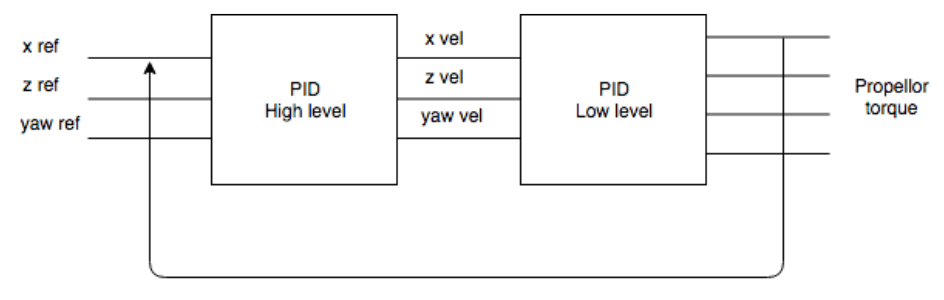
\includegraphics[width=12cm]{controller.png}
		\caption{Cascaded controller overview\label{Cascaded controller overview}}
	\end{figure}
	
	